\documentclass[conference,9pt]{IEEEtran}
\usepackage{xcolor}
\usepackage{cite}
\usepackage{epsfig}
\usepackage{amssymb}
\usepackage{amsmath}
\usepackage{graphicx}
\graphicspath{ {./} }

\begin{document}
\title{Practical 4b}

\author{
\IEEEauthorblockN{Albert Acebron}
\IEEEauthorblockA{NIU: 1458626}
}

\maketitle
\begin{abstract}
In this practical we will use an adaptive filter based on the LMS algorithm developed before to filter out the unwanted signal in our data.
\end{abstract}

\section{Questions}

\subsection{Question 1}
Combining equations (1.2) and (1.3) we get:

$$\frac{\sum b_k z^{-k}}{1 + \sum a_k z^{-k}} = K\frac{1-2cos(\omega_{int})z^{-1} + z^{-2}}{1- 2rcos(\omega_{int})z^{-1}+r^2z^{-2}}$$

So if we solve this equation for the coefficients we'll get that:
$$b_0=1$$
$$b_1=-2cos(\omega_{int})$$
$$b_2=1$$
$$a_0=1$$
$$a_1=-2rcos(\omega_{int})$$
$$a_2=r^2$$

Using this we can calculate the value of $K$:
$$K=\frac{1 + a_1+a_2}{b_0+b_1+b_2}=\frac{1-2rcos(\omega_{int})+r^2}{1-2cos(\omega_{int})+1}$$

If we now take a look at the periodogram of the practical 3:

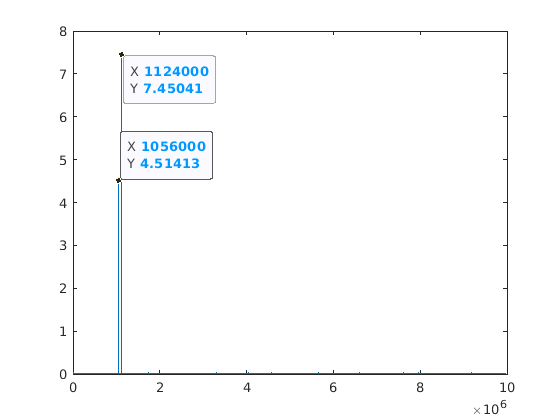
\includegraphics[scale=0.6]{perio.png}

We can calculate $\omega_{int}$ using the frequency of the inteferring signal:
$$\omega_{int}=\frac{2\pi \cdot 1.124 MHz}{10 MHz} = 0.7062$$

And then proceed to graph the impulsional response of the filter (initially using $r=1.5$):

\begin{verbatim}
  wint = 0.7062;
  r=1.5;
  K=(1-2*r*cos(wint)+r^2)/(1-2*cos(wint)+1);
  w=0:pi/1000:pi;
  z=exp(j*w);
  H=K*(1-2*cos(wint)*z.^(-1)+z.^(-2))
   ./(1-2*r*cos(wint)*z.^(-1)+r^2*z.^(-2));
  % Plot
  plot(w, 10*log(abs(H)));
\end{verbatim}

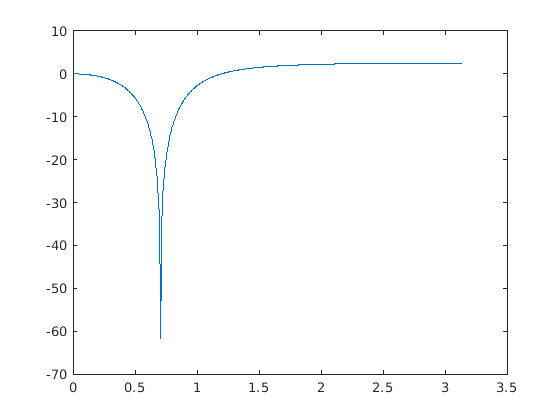
\includegraphics[scale=0.6]{filter-response.png}

And if we now overlap it with the tones of the signal:

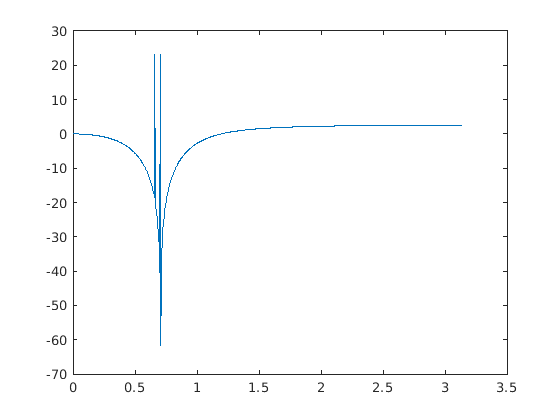
\includegraphics[scale=0.6]{complete-filter-res.png}

As we can see, the filter is correctly filtering our interferring signal, but the other signal is also getting caught up in it. To fix that we'll set $r=1.15$:

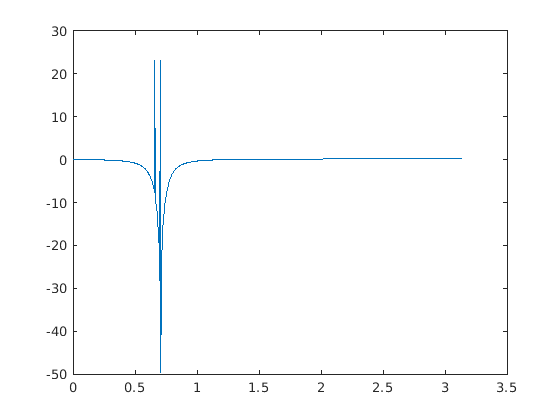
\includegraphics[scale=0.6]{r1-1.png}

Now the filter is much more selective and, although it still reduces our wanted signal, the reduction is much lower.

\subsection{Question 2}
Let's apply the notch filter we constructed to get rid of the unwanted signal, to do so we'll calculate the filter coefficients and use filter():
\begin{verbatim}
  r=1.15
  a=[r^2, -2*r*cos(wint), 1]
  b=[1, -2*cos(wint), 1]*K
  filtered=filter(b, a, RxSignal)
  per = compute_periodogram(filtered)
  plot(linspace(0, 1e7, length(per)), per)
\end{verbatim}

Which results in a signal that has the following periodogram:

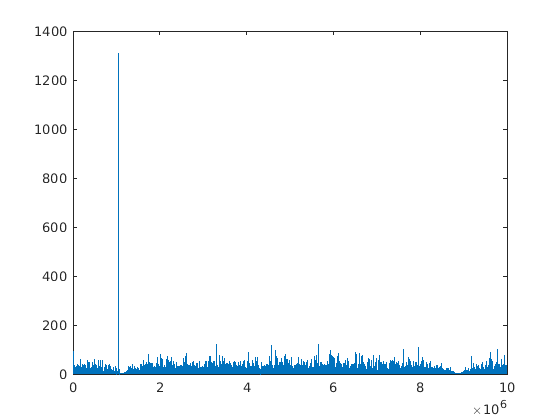
\includegraphics[scale=0.6]{filtered.png}

As we can appreciate, the unwanted signal has been completely removed.

\subsection{Question 3}
Next, we'll try to use an adaptive filter to simulate the notch filter developed before. This will be done by using the filtered signal from before as our reference signal $d(n)$ and minimizing the error $e(n)$:

\begin{verbatim}
  [Hf, y, e]=algoritmeLMS(filtered, RxSignal,
     60, 1e-5);
  per = compute_periodogram(y)
  plot(linspace(0, 1e7, length(per)), per)
\end{verbatim}

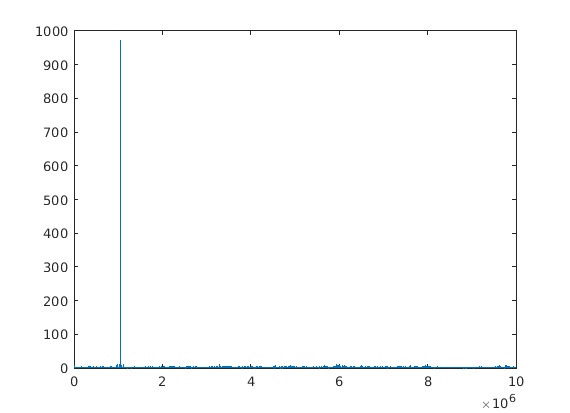
\includegraphics[scale=0.6]{filtered-lms.png}

The signal at the interferring frequency has been removed, so the filter is working well.

\subsection{Question 4}
If we now proceed to graph the frequency response of the last iteration of the adaptive filter (we've chosen the last iteration because it should be the best one), we'll see the following result:

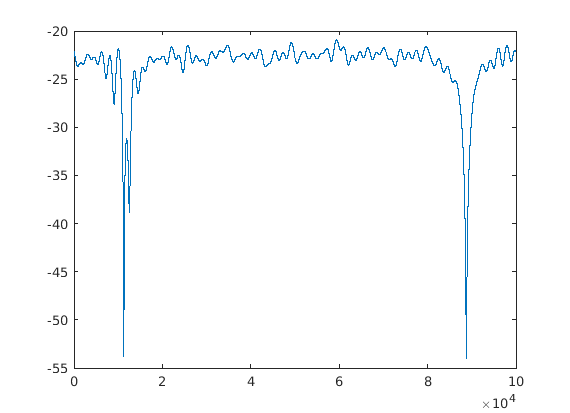
\includegraphics[scale=0.6]{freq-response.png}

As we can expect, the filter has evolved to heavily reduce the signal at the interferring frequency, but also surprisingly we see a notch on the other side of the spectrum that mitigates signals at that frequency. The reason behind this second notch is that, if we look closely at the periodogram of the filtered signal we got on question 2, we'll see that the frequencies on the same spot at the right end of the spectrum got reduced as well, so LMS has replicated that part of the filtering as well by adding a second notch there.

If we want to dig deeper, the reason why frequencies on that spot in the right side of the spectrum got reduced is that, in the construction of the notch filter, we apply the cosine function to $w_{int}$, which represents the inteferring frequency. $cos$ has the property that $cos(x)=cos(-x)$ so we'll get the same filter whether our interferring frequency is $w_{int}$ or $2\pi-w_{int}$, meaning that the filter must mitigate both of those frequencies to work effectively.

\subsection{Question 5}
If we wish to obtain the impulsional response of our notch filter there are several ways to go around it. For example, we could obtain it by operating on the EDF equation defined on (1.1), but an easier way to calculate that value is by applying the definition of impulsional response, that is the output signal of a system through which a dirac delta has been sent.

So we'll just construct a dirac delta (that has a number of points equal to the amount of coefficients used in LMS, as the practical requires the response to have the same amount of points) and apply our filter to it with filter(), as we did previously.

\begin{verbatim}
  d=zeros(60, 1);
  d(1)=1e5;
  resp=filter(b, a, d);
  plot(resp)
\end{verbatim}

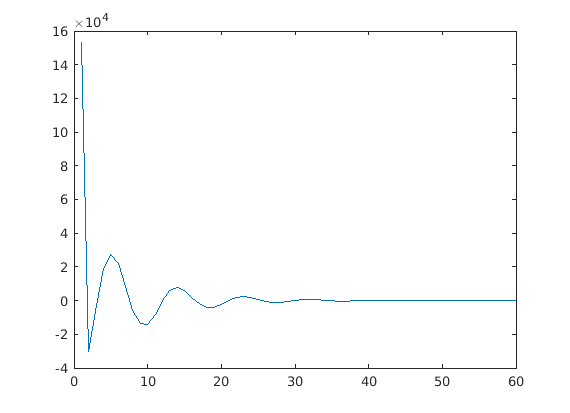
\includegraphics[scale=0.6]{imp-resp.png}

\subsection{Question 6}
Let's compare this result with the impulsional response of the filter derived from LMS (concretely the one from the last iteration). In this case the coefficients already represent the impulsional response so we can just use those directly:
\begin{verbatim}
  plot(abs(Hf(:,length(Hf))))
\end{verbatim}

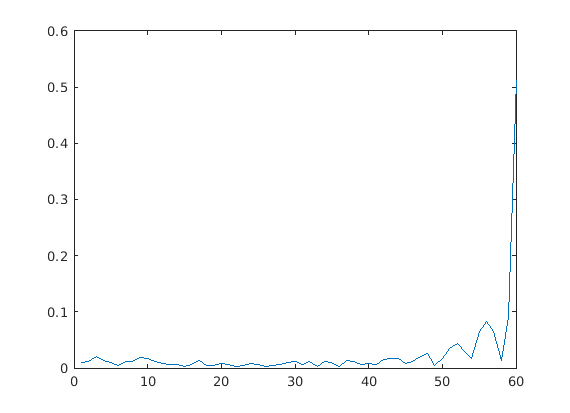
\includegraphics[scale=0.6]{im-lms.png}

If we compare this against the absolute value of the impulsional response of the notch filter:

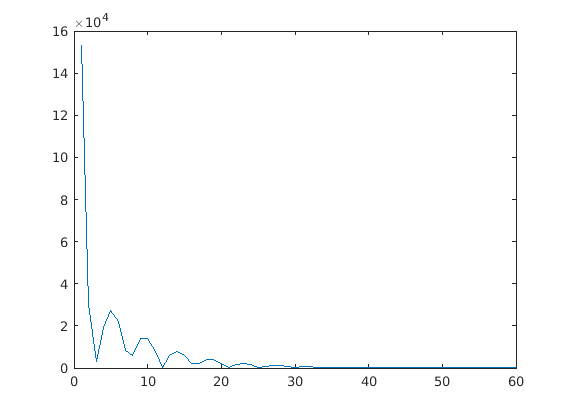
\includegraphics[scale=0.6]{im-abs.png}

We can appreciate that, ignoring the scale difference (this is just caused by the value of the delta that we applied, which is arbitrary since we can't create a perfect delta and are forced to use an approximation), both impulse responses are extremely similar but are time reversed against the other.

These being similar is what we would expect, as, after all, the LMS-derived filter is just trying to imitate the notch filter, so if it does it's job well the coefficients of the filter should end up being extremely similar, as the filter is replicated.

The time reversal is unexpected though, but it's existence can be explained with the time reversal property of the fourier transform, which says that if the fourier transform is applied to a time-reversed function the resulting function will be a conjugated version of what we would get if we applied the transform to a non-time-reversed version of the same function, in other words $F(h(-t))=H*(f)$.

Now, when we compute the periodogram we are calculating $|F(h)|^2$, which provides the same results whether F is conjugated or not ($|H|^2$=$|H*|^2$), so putting together these two facts we can conclude that the periodogram will be the same if our filter has been time reversed ($|F(h(-t))|^2=|H*|^2=|H|^2=|F(h(t))|^2$). Thus, the property of reducing the interferring signal will hold true if the impulsional response has been time-reversed.

Putting it all together, we conclude that the impulsional responses of the two filters are extremely similar and fulfill it's objectives well, which is what we wanted since the LMS-based filter is imitating the other one.

\subsection{Question 7}
The LMS algorithm goes through 4942 iterations, so we'll look at the first coefficient of the filter in several of these and compare it against the one in the notch filter it's trying to imitate in order to trace it's evolution through time:

\begin{verbatim}
  notch=resp(1)
  it=zeros(5,1)
  it(1)= Hf(60,10)-notch
  it(2)=Hf(60,100)-notch
  it(3)=Hf(60,500)-notch
  it(4)=Hf(60,2000)-notch
  it(5)=Hf(60,end)-notch
  plot([10, 100, 500, 2000, length(Hf)], abs(it))
\end{verbatim}

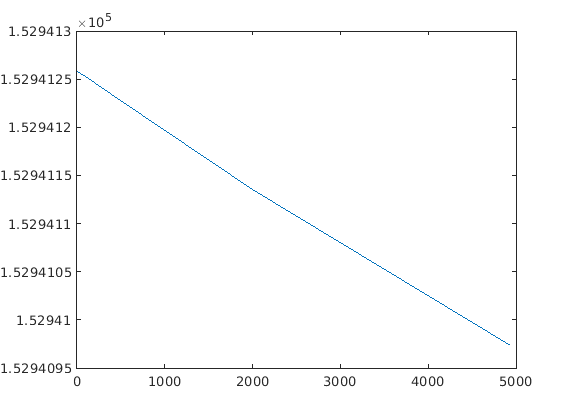
\includegraphics[scale=0.6]{error-evolution.png}

As we can see, with an increase in iterations the LMS filter gets closer to the notch one. This makes sense, since LMS is just optimizing it's filter to become similar to the other one, so the more iterations the algorithm runs the better the optimization will be and thus the closer the filter will be to the one it's trying to imitate, driving the error to zero.

An interesting experiment to try here is to apply the LMS algorithm with multiple possible values of $\mu$, because that defines the step size used in the optimization, thus we should theoretically see that if we increase the step size the speed at which the error goes down increases (with a few caveats, for example if the step size ends up continuously overshooting the minimum we might end up with a lower rate of descent or no convergence), as each iteration will move a larger distance towards the minimum.

This can be seen in the following graph, which contains multiple values of $\mu$ (blue: 1e-5, red: 1e-4, yellow: 1e-10):

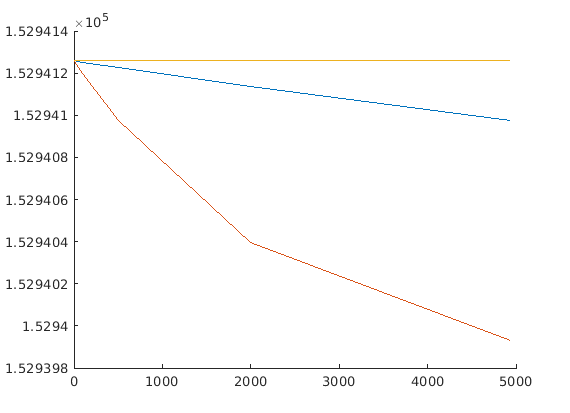
\includegraphics[scale=0.6]{mus.png}

The previous graph proves that what we theorized holds true and higher learning rates/values of $\mu$ lead to faster reduction of the error.

\section{Appendix}
\subsection{Add tones to filter response graph}
\begin{verbatim}
  H(round(1124000/5e6*length(H)))=10;
  H(round(1056000/5e6*length(H)))=10;
\end{verbatim}

\subsection{Graph frequency response of adaptive filter}
\begin{verbatim}
  plot(10*log10(compute_periodogram(Hf(:,
   length(Hf)))))
\end{verbatim}

\subsection{Plot absolute impulsional response}
\begin{verbatim}
  plot(abs(resp))
\end{verbatim}

\subsection{Plot error through iterations for multiple $\mu$}
Repeat the following code for multiple values of mu:
\begin{verbatim}
  mu = 1e-5
  [Hf, y, e]=algoritmeLMS(filtered, RxSignal, 60, mu);
  notch=resp(1)
  it=zeros(5,1)
  it(1)= Hf(60,10)-notch
  it(2)=Hf(60,100)-notch
  it(3)=Hf(60,500)-notch
  it(4)=Hf(60,2000)-notch
  it(5)=Hf(60,end)-notch
  plot([10, 100, 500, 2000, length(Hf)], abs(it))
\end{verbatim}

\end{document}


